\documentclass[12pt,letterpaper]{article}
\usepackage{amsmath}
\usepackage{amsfonts}
\usepackage{amsthm}
\usepackage{mathtools}
\usepackage{cancel}
\usepackage[margin=1in]{geometry}
\usepackage{titling}
\usepackage{fp}
\usepackage{enumitem}
\usepackage[super]{nth}
\usepackage{dcolumn}
\usepackage{minted}
\usepackage[title]{appendix}
\usepackage{pgfplots}
\pgfplotsset{compat=1.8}
\usepgfplotslibrary{statistics}
\usepackage[round-mode=figures,round-precision=3,scientific-notation=false]{siunitx}

\newcolumntype{d}{D{.}{.}{-1}}

\setlength{\droptitle}{-10ex}

\preauthor{\begin{flushright}\large \lineskip 0.5em}
\postauthor{\par\end{flushright}}
\predate{\begin{flushright}\large}
\postdate{\par\end{flushright}}

\title{STA 032 R Final\vspace{-2ex}}
\author{Hardy Jones\\
        999397426\\
        Professor Melcon\vspace{-2ex}}
\date{Winter 2015}

\begin{document}
  \maketitle

  \newmintedfile[rData]{r}{ fontsize=\footnotesize
                          , frame=single
                          }

  \begin{enumerate}
    \item
      \begin{enumerate}
        \item $P(Z)$

          \begin{tabular}{| r | d |}
            \hline
            n     & \multicolumn{1}{c |}{probability} \\
            \hline
            \num{10000}  & 0.3240 \\
            \hline
            \num{100000} & 0.3300 \\
            \hline
          \end{tabular}
        \item $P(T)$

          \begin{tabular}{| r | d |}
            \hline
            n     & \multicolumn{1}{c |}{probability} \\
            \hline
            \num{10000}  & 0.3220 \\
            \hline
            \num{100000} & 0.3190 \\
            \hline
          \end{tabular}
        \item $P(P)$

          \begin{tabular}{| r | d |}
            \hline
            n     & \multicolumn{1}{c |}{probability} \\
            \hline
            \num{10000}  & 0.3540 \\
            \hline
            \num{100000} & 0.3510 \\
            \hline
          \end{tabular}
        \item $P(M|Z)$

          \begin{tabular}{| r | d |}
            \hline
            n     & \multicolumn{1}{c |}{probability} \\
            \hline
            \num{10000}  & 0.7760 \\
            \hline
            \num{100000} & 0.7860 \\
            \hline
          \end{tabular}
        \item $P(M^c|P^c)$

          \begin{tabular}{| r | d |}
            \hline
            n     & \multicolumn{1}{c |}{probability} \\
            \hline
            \num{10000}  & 0.3060 \\
            \hline
            \num{100000} & 0.2970 \\
            \hline
          \end{tabular}
        \item $P(Z\cap M^c)$

          \begin{tabular}{| r | d |}
            \hline
            n     & \multicolumn{1}{c |}{probability} \\
            \hline
            \num{10000}  & 0.0724 \\
            \hline
            \num{100000} & 0.0705 \\
            \hline
          \end{tabular}
        \item $P(T\cup M)$

          \begin{tabular}{| r | d |}
            \hline
            n     & \multicolumn{1}{c |}{probability} \\
            \hline
            \num{10000}  & 0.7680 \\
            \hline
            \num{100000} & 0.7740 \\
            \hline
          \end{tabular}
      \end{enumerate}
    \item
      \begin{enumerate}
        \item $\theta_A$

          \begin{tabular}{| d | d |}
            \hline
            \multicolumn{1}{| c |}{estimate} & \multicolumn{1}{c |}{error} \\
            \hline
            0.9810                         & 0.0572 \\
            \hline
          \end{tabular}
        \item $\theta_B$

          \begin{tabular}{| d | d |}
            \hline
            \multicolumn{1}{| c |}{estimate} & \multicolumn{1}{c |}{error} \\
            \hline
            0.1480                         & 0.0236 \\
            \hline
          \end{tabular}
        \item $\theta_C$

          \begin{tabular}{| d | d |}
            \hline
            \multicolumn{1}{| c |}{estimate} & \multicolumn{1}{c |}{error} \\
            \hline
            4.710                          & 0.417 \\
            \hline
          \end{tabular}
      \end{enumerate}
    \item
      \begin{enumerate}
        \item
          \begin{enumerate}
            \item
              \begin{tabular}{| l | d | d |}
                \hline
                            & \multicolumn{1}{c |}{Lower} & \multicolumn{1}{c |}{Upper} \\
                \hline
                Corrected   & 0.685                       & 0.871 \\
                \hline
                Uncorrected & 0.707                       & 0.893 \\
                \hline
              \end{tabular}
            \item
              \begin{tabular}{| l | d | d |}
                \hline
                            & \multicolumn{1}{c |}{Lower} & \multicolumn{1}{c |}{Upper} \\
                \hline
                Corrected   & 0.240                       & 0.543 \\
                \hline
                Uncorrected & 0.229                       & 0.540 \\
                \hline
              \end{tabular}
          \end{enumerate}
        \item
          \begin{enumerate}
            \item
              \begin{tabular}{| d | d |}
                \hline
                \multicolumn{1}{| c |}{Corrected} & \multicolumn{1}{c |}{Uncorrected} \\
                \hline
                0.9614 & 0.9329 \\
                \hline
              \end{tabular}
            \item
              \begin{tabular}{| d | d |}
                \hline
                \multicolumn{1}{| c |}{Corrected} & \multicolumn{1}{c |}{Uncorrected} \\
                \hline
                0.9475 & 0.9475 \\
                \hline
              \end{tabular}
            \item
              \begin{tabular}{| d | d |}
                \hline
                \multicolumn{1}{| c |}{Corrected} & \multicolumn{1}{c |}{Uncorrected} \\
                \hline
                0.9601 & 0.9445 \\
                \hline
              \end{tabular}
            \item
              \begin{tabular}{| d | d |}
                \hline
                \multicolumn{1}{| c |}{Corrected} & \multicolumn{1}{c |}{Uncorrected} \\
                \hline
                0.9362 & 0.9362 \\
                \hline
              \end{tabular}
          \end{enumerate}
        \item
          The difference is large enough that using the corrected version makes sense.
          It does not add more asymptotic complexity,
          but it provides a greater coverage probability.
          You basically get better coverage for free.
        \item
          The true proportion affects the uncorrected version more than the corrected version.
          The sample size does not really affect either version.
        \item
          The corrected version can have worse coverage when the true mean is very low and the sample size is very large.
        \item
          Given the results of (d) and (e), it would depend on the situation.
          If the sample size is very large and the true mean is very small then it would be better to use the uncorrected version.
          If not, it's better to use the corrected version.
      \end{enumerate}
    \item
      We start by generating a histogram:

      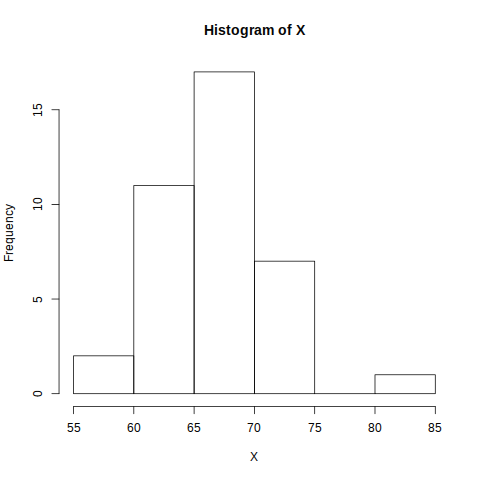
\includegraphics[width=\linewidth]{prob4.png}

      The data appears to be distributed approximately normally.

      \begin{enumerate}
        \item $\mu_0 = 67$

          \begin{tabular}{| d | d | d |}
            \hline
            \multicolumn{1}{| c |}{Non-parametric} & \multicolumn{1}{c |}{Parametric} & \multicolumn{1}{c |}{Theoretical} \\
            \hline
            0.637 & 0.627 & 0.629 \\
            \hline
          \end{tabular}
        \item $\mu_0 = 68$

          \begin{tabular}{| d | d | d |}
            \hline
            \multicolumn{1}{| c |}{Non-parametric} & \multicolumn{1}{c |}{Parametric} & \multicolumn{1}{c |}{Theoretical} \\
            \hline
            0.146 & 0.151 & 0.153 \\
            \hline
          \end{tabular}
        \item $\mu_0 = 69$

          \begin{tabular}{| d | d | d |}
            \hline
            \multicolumn{1}{| c |}{Non-parametric} & \multicolumn{1}{c |}{Parametric} & \multicolumn{1}{c |}{Theoretical} \\
            \hline
            0.00628 & 0.00849 & 0.00863 \\
            \hline
          \end{tabular}
      \end{enumerate}
  \end{enumerate}

  \begin{appendices}
    \section{R code}

        \subsection*{Problem 1}
            \rData{prob1.R}
            \subsubsection*{(a)}
                \rData{prob1a.R}
            \subsubsection*{(b)}
                \rData{prob1b.R}

        \subsection*{Problem 2}
            \rData{prob2.R}
            \subsubsection*{(a)}
                \rData{prob2a.R}
            \subsubsection*{(b)}
                \rData{prob2b.R}

        \subsection*{Problem 3}
            \rData{prob3.R}
            \subsubsection*{(a)}
                \rData{prob3a.R}
            \subsubsection*{(b)}
                \rData{prob3b.R}

\end{appendices}


\end{document}
